\section{Literature Review}

\label{sec:literatureReview}

% Iowa Electronic Markets
% PredictIt, PredictAlot
% Intrade
% Rational expectations - demand not same as traditional market
% PredictIt disputes: wording

\subsection{The Iowa Electronic Markets}

The Iowa Electronic Markets (IEM) are real-money prediction markets developed
by the University of Iowa~\cite{IEM} that have been running since 1988. They
allow users to buy and sell contracts based on the outcome of U.S. political
elections and economic indicators, and are currently offering markets for the
winning party of the 2020 U.S. presidential election, the vote share between
the Democratic and Republican parties in the 2020 U.S. presidential election,
and the compositions of the houses of Congress, House of Representatives, and
U.S. Senate after the outcome of the 2020 U.S. congressional elections. The
number of markets offered is small and the topics are kept relevant to current
events, meaning there is likely to be high liquidity for any security a user
wishes to trade in. This has allowed the markets to predict the results of
political elections with more accuracy and less error than traditional polls:
for the presidential elections between 1988 and 2000, three-quarters of the
time the IEM's market price on the day each poll was released was more accurate
for predicting vote share than the poll itself~\cite[pg.~19]{WisdomOfCrowds}.
These markets inspired similar markets in the forms of the Hollywood Stock
Exchange, NewsFutures, and the Foresight Exchange report, which achieved
similar successes despite not using real money. 

\subsection{Combinatorial Markets}

An issue with these markets is that they are restrictive in the bets they
offer. Although this can be beneficial in that they provide a focused and
liquid market in which to trade, they are less expressive. A combinatorial
prediction market drastically increases the number of outcomes that can be
predicted by offering securities on propositions that can be combined in
various ways. One example of such a market is
\emph{Predictalot}~\cite{Predictalot}, a combinatorial prediction market
developed by Yahoo! that allowed users to trade securities in the 2010 NCAA
Men's Division I Basketball Tournament. The tournament sees the top 64 teams
play 63 games in a knockout competition, yielding a total outcome space of size
$2^{63}$. \emph{Predictalot} then kept track of the odds, computing them by
scanning through all of the predictions made by users. This application served
as the original inspiration for this project to explore prediction markets.
Using a Market Scoring Rule for such a market would involve computing a
summation over the entire outcome space $\Omega$, an intractable, \#P-hard
problem akin to counting the number of subsets in a list of integers that sum
to zero. Instead, they use importance sampling, a technique for estimating
properties of a particular probability distribution using only samples
generated from a different distribution. This ``naive'' approach is then
improved upon by the work of Dud\'ik, Lahaie, and Pennock~\cite{Dudik2012}, who
use convex optimisation and constraint generation to develop a tractable market
maker. This approach is a compromise between treating all securities as
independent and a fully combinatorial, ``ideal'' market maker, but still allows
for information to be gathered among related securities. This allows for them
to compute odds that make sense: for example, a large bet on a team to win the
entire tournament would also increase their odds at every other stage in the
tournament, since they must win these to even reach the final. Kroer, Dud\'ik,
Lahaie, and Balakrishnan~\cite{Kroer2016} use integer programming to remove
trades which are always profitable and incur no risk. In other words, they
ensure all trades are arbitrage-free. On top of achieving bounded loss, a
crucial element behind a market mechanism operating in the real world and
avoiding bankruptcy, avoiding arbitrage is desirable as it leads to more
accurate forecasts: since users cannot make risk-free profits, they are forced
to bet according to their true beliefs.

\subsection{Decentralised Markets}

All examples so far have involved a centralised market mechanism. These types
of systems involve a central authority providing the securities upon which
users may trade and then verifying their outcome. \emph{Decentralised} markets
allow the users to specify the securities themselves and trade shares in them.
Several examples of decentralised markets exist, and they are often implemented
with cryptocurrencies. Peterson et al.~\cite{Peterson2015} study the setting
and implement the oracle at the heart of \emph{Augur}~\cite{Augur}, a
decentralised prediction market built upon the Ethereum blockchain, which
launched in 2018. It allows users to offer predictions on any topic, and
markets may be either categorical, which are similar to binary markets in which
the winner takes all, or scalar, which offer users a spectrum of outcomes in
which to invest. As in many decentralised markets, outcomes of events are then
resolved by the users, and in \emph{Augur} users are incentivised to report
truthfully by way of paying reporting fees: users back their report by
depositing tokens, and token holders are then entitled to the trading fees
generated.  Although this persuades against manipulation, it has not been shown
whether this system achieves any theoretical guarantees of truthful reporting.

As can often be the case with real-money markets, the platform had quickly
devolved into an assassination market~\cite{AugurDeathMarket} -- originally
this referred to the case where users created markets on the deaths of certain
people, which then incentivised their assassination. A user could stand to
profit by placing a bet on the exact time of their death, and ensure this bet
was profitable by assassinating the subject. More generally this refers to the
users of a prediction market having the ability to influence a market's outcome
and acting on this opportunity. Another issue with \emph{Augur} is the option
to report a market's outcome as ``invalid'': this is for the case where the
user-made bet is too ambiguous to decided, such as, ``Bayern Munich will play
well against Paris Saint Germain''.

Other decentralised markets based on cryptocurrencies exist, including
\emph{Omen}~\cite{Omen} and \emph{Hivemind}~\cite{Hivemind}. The former is
similar to \emph{Augur} in that it allows users to create markets for any bet
they like and whose outcomes are not decided by the system itself. Whereas
\emph{Augur} uses a reputation system whereby users back their report of a
market's outcome with \$REP tokens, \emph{Omen} asks the market creator to
supply an ``oracle'' through which the outcome can be determined. This oracle
can even be \emph{Augur}. Although this may solve the ``invalid'' outcome
option for ambiguous bets, it may introduce bias into the process of outcome
determination. For example, suppose a user creates a market for ``The
Democratic nominee will tell a lie during tonight's debate'' and lists the
oracle as the conservative news channel, Fox News. Users would then trade on
how they think the oracle will report the outcome, and not what they believe
the outcome will be themselves. An important aspect of decentralised markets
must therefore be that the outcome is determined by the community, not a single
source. 

In contrast to \emph{Augur}, which implements a traditional order book using
Ethereum, \emph{Omen} uses an automated market maker to provide liquidity to
its securities. As we have discussed, automated market makers can be
implemented via Market Scoring Rules. Hanson~\cite{Hanson2003} shows that we
can use any strictly proper scoring rule to implement an automated market
maker: with such scoring rules, agents maximise their expected utility by
truthfully revealing their predictions. In particular, in this project we
implement the peer prediction market introduced by Freeman, Lahaie, and
Pennock~\cite{Freeman2017}, which specifies a mechanism to trade bets and
crowdsource outcome determination. Market outcomes are decided by asking users
for reports, similarly to \emph{Augur}. All they require is that the rule is
strictly proper, giving plenty of choice to study the effects different rules
have on user and price behaviour. While the choice of scoring rule is less
important than the mechanism by which market outcomes are determined, a recent
work by Liu, Wang, and Chen~\cite{Liu2020} introduces scoring rules for the
setting where the aggregator has access only to user reports, which they call
Surrogate Scoring Rules (SSRs). This appears to be an interesting avenue to
further explore and adapt to a prediction market. One assumption they make,
however, seems incompatible with the decentralised setting in that they require
all events to be independent.  Given that users can create a market for
\emph{any} bet, this condition is impossible to ensure. Since SSRs can be
strictly proper under certain conditions, they may be suitable as the Market
Scoring Rule in \cite{Freeman2017}. 

Other prediction markets existed in \emph{PredictIt}~\cite{PredictIt} and
\emph{InTrade}~\cite{InTrade}, both offering markets for various political and
economic events. However, both experienced disputes largely related to the
wording of the available to trade and the ambiguity in their resolution. For
example, a bet offered on \emph{PredictIt} was, ``Who will be Senate-confirmed
Secretary of State on March 31, 2018?'', and although Rex Tillerson was fired
in the middle of March, he was officially the secretary of state until midnight
of the 31st, leading to confusion among users in what they are trading on and
therefore inaccuracies in the predictions it elicited. This will be a problem
inherent to any prediction market that allows users to specify their own bets,
and while the work of Freeman et al.~\cite{Freeman2017} mitigates the problem of
determining the outcome by setting it to the proportion of users reporting a
``yes'' outcome, this does nothing to penalise the initial creator for
introducing an ambiguous market.

\begin{figure}[h]
	\centering
	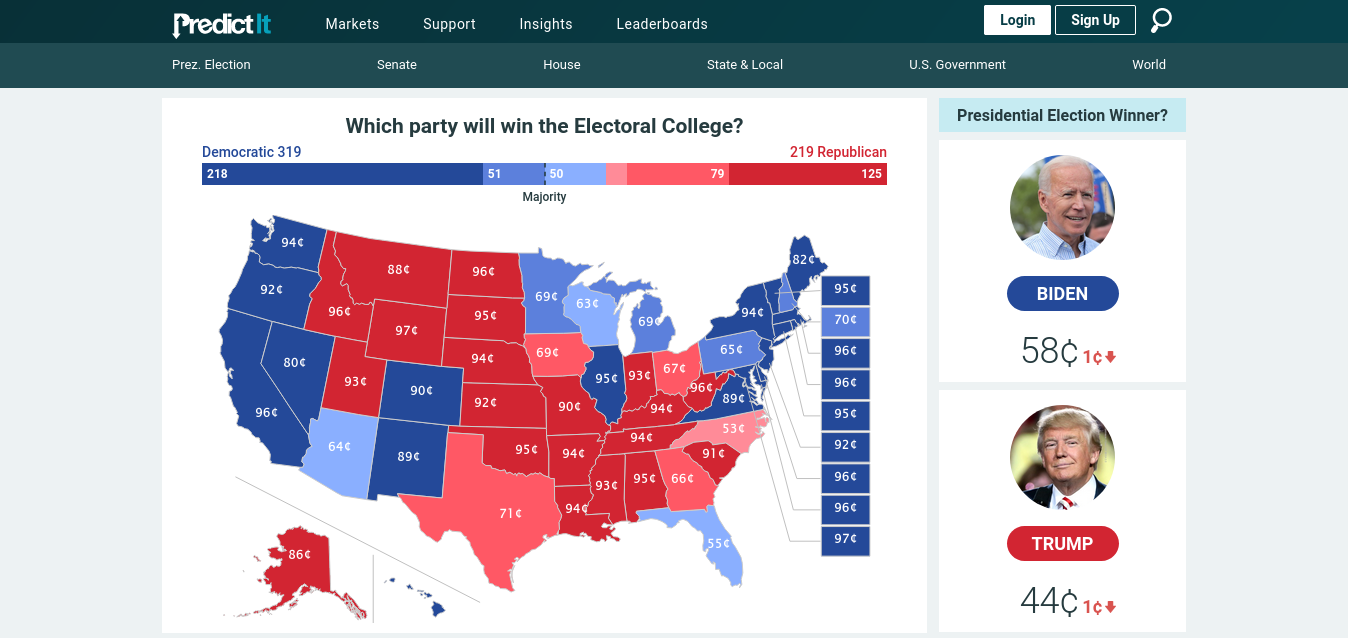
\includegraphics[width=\textwidth]{predictit}
	\caption{The \emph{PredictIt} prediction market for the 2020 U.S.
	presidential election. As of \today\ Joe Biden is perceived to be more
	likely to become President.}
	\label{fig:predictit}
\end{figure}

\subsection{A Note on \emph{Predictalot}}

As we will cover in the following section, the goals of this project are more
concerned with the game-theoretic aspects of implementing a decentralised
prediction market. This involves encouraging users to act in the desired
manner, which in our case means ``telling the truth'' about both their beliefs
on an event's outcome and their observation of the result. Since combinatorial
prediction markets are often centralised, meaning bets come straight from the
system and not its users, all users have to do is choose to participate in the
market at what they view as the correct price, hence there is much less
opportunity for manipulation. For this reason, combinatorial prediction markets
are more concerned with the computational aspects of offering combinatorial
securities to its traders, and in particular how to compute accurate prices on
combinations of interrelated securities. Both decentralised and combinatorial
settings are interesting in their own right, and both can achieve an added
level of expressiveness compared to a traditional prediction market such as the
IEM. Here we will briefly describe approaches taken to improving the efficiency
of pricing in the \emph{Predictalot} prediction market.

We will first discuss the hardness of using a Market Scoring Rule to calculate
prices in a combinatorial market. The class NP is the set of decision problems
for which, given an input to the problem and a proposed solution, the
``certificate'', verification that the certificate is indeed a correct solution
can be done in polynomial time. By self-reducibility, the search version of the
problem is no harder than the decision version. The class \#P consists of
\emph{functions} that count the number of solutions to NP search problems. A
function $g$ is \#P-hard if, for every function $f$ in \#P, given an oracle for
$g$ we can compute $f$ in polynomial time -- that is, computing $g$ is at least
as hard as any other function $f$ in \#P. Chen et al.~\cite{Chen2008} show that
computing the price and cost functions of a MSR in a combinatorial market is
\#P-hard, even when traders are restricted to betting on the disjunctions or
conjunctions of two events. They do this via a reduction to the \#P-hard
function \textsc{\#2-SAT}, which counts the number of satisfying assignments of
a CNF formula, where each clause has two literals. 

Dud\'ik et al.~\cite{Dudik2012} restrict the bidding language to achieve
tractability. This is done by firstly calculating prices as if markets were
independent then detecting and minimising arbitrage. Opportunities for arbitrage
are detected using constraint generation, in which arbitrage occurs when the
price falls below a certain level, and this is minimised using optimisation
methods. This does not always completely remove all arbitrage opportunities.
Kroer et al.~\cite{Kroer2016} apply a similar approach by interleaving the
execution of trades with the removal of arbitrage via constraint generation,
and in fact use the method of Dud\'ik et al., their \emph{Linear Constraint
Market Maker (LCMM)}, in order to first remove ``easy'' arbitrage prices. They then
feed their generated integer program (IP) constraints to an algorithm which
attempts to solve it. Since solving IPs is NP-hard, and with such a large
outcome space there may not be time to solve the IP in time before a new trade
is submitted, in which case they interrupt this step. Regardless of whether it
was interrupted, they guarantee non-negative profit for every trade. When
tested on data from \emph{Predictalot}, they found an improvement in the
accuracy of their odds over those computed by the LCMM alone, and allowing 30
minutes to solve the IPs yielded trades that could execute in 5 hours, that
originally took 22 days. This shows the huge computational task involved in
computing accurate prices in combinatorial markets, and they identify that
further speedup can be obtained by not solving the IPs optimally, but instead
using local search to find solutions that are ``good enough''.
